% !TEX program = pdflatex
\documentclass[11pt,a4paper]{article}

\usepackage[T1]{fontenc}
\usepackage[utf8]{inputenc}
\usepackage{lmodern}
\usepackage{microtype}
\usepackage[margin=1in]{geometry}
\usepackage{amsmath,amssymb,amsthm}
\usepackage{mathtools}
\usepackage{booktabs}
\usepackage{tabularx}
\usepackage{array}
\usepackage{enumitem}
\usepackage{xcolor}
\usepackage{listings}
\usepackage{tikz}
\usetikzlibrary{arrows.meta,positioning,fit,shapes.geometric,calc}
\usepackage[hidelinks,colorlinks=true,linkcolor=blue!50!black,citecolor=blue!50!black,urlcolor=blue!50!black]{hyperref}
\usepackage{cleveref}
\usepackage{framed}

% Loosen line-breaking so long inline identifiers don't overflow.
\sloppy

% ---- macros ----------------------------------------------------------------
\newcommand{\G}{\mathbb{G}}
\newcommand{\Zq}{\mathbb{Z}_q}
\newcommand{\sk}{\mathit{sk}}
\newcommand{\pk}{\mathit{pk}}
\newcommand{\Hzero}{H_0}
\newcommand{\Hone}{H_1}
\newcommand{\Htwo}{H_2}
\newcommand{\sample}{\xleftarrow{\$}}
\newcommand{\Sign}{\textsf{Sign}}
\newcommand{\Verify}{\textsf{Verify}}
\newcommand{\Trace}{\textsf{Trace}}
\newcommand{\KeyGen}{\textsf{KeyGen}}
\newcommand{\file}[1]{\texttt{#1}}

% Boxes for sidebars
\definecolor{boxbg}{rgb}{0.96,0.97,0.99}
\definecolor{boxrule}{rgb}{0.30,0.40,0.55}
\newenvironment{intuition}[1][Intuition]{%
  \def\FrameCommand{\fboxsep=8pt\fcolorbox{boxrule}{boxbg}}%
  \MakeFramed{\advance\hsize-2\fboxsep\FrameRestore}%
  \noindent\textbf{#1.}\par\smallskip%
  \itshape
}{\endMakeFramed}

\definecolor{flagbg}{rgb}{0.99,0.96,0.92}
\definecolor{flagrule}{rgb}{0.65,0.40,0.10}
\newenvironment{flagbox}[1][Heads up]{%
  \def\FrameCommand{\fboxsep=8pt\fcolorbox{flagrule}{flagbg}}%
  \MakeFramed{\advance\hsize-2\fboxsep\FrameRestore}%
  \noindent\textbf{#1.}\par\smallskip%
}{\endMakeFramed}

\theoremstyle{definition}
\newtheorem{flaw}{Issue}

% ---- listings --------------------------------------------------------------
\definecolor{codebg}{rgb}{0.97,0.97,0.97}
\lstdefinestyle{py}{
  language=Python,
  basicstyle=\ttfamily\small,
  backgroundcolor=\color{codebg},
  frame=single,framesep=4pt,
  rulecolor=\color{black!15},
  keywordstyle=\color{blue!60!black}\bfseries,
  stringstyle=\color{green!30!black},
  commentstyle=\color{gray}\itshape,
  showstringspaces=false,breaklines=true,
}
\lstdefinestyle{shell}{
  basicstyle=\ttfamily\small,
  backgroundcolor=\color{codebg},
  frame=single,framesep=4pt,
  rulecolor=\color{black!15},
  breaklines=true,breakatwhitespace=true,
  postbreak=\mbox{\textcolor{gray}{$\hookrightarrow$}\space},
  showstringspaces=false,
}
\lstdefinestyle{json}{
  basicstyle=\ttfamily\footnotesize,
  backgroundcolor=\color{codebg},
  frame=single,framesep=4pt,
  rulecolor=\color{black!15},
  showstringspaces=false,breaklines=true,
}
\lstdefinestyle{pseudo}{
  basicstyle=\ttfamily\small,
  backgroundcolor=\color{codebg},
  frame=single,framesep=4pt,
  rulecolor=\color{black!15},
  showstringspaces=false,breaklines=true,
  mathescape=true,
}

\title{\textbf{Engineering Notes:\\ e-ring-voting v0.3}\\[0.4em]
       \large Onboarding for a new collaborator}
\author{Daniele Lin \and Niccol\`o Pagano}
\date{May 2026}

\begin{document}
\maketitle

\begin{quote}
\itshape
These notes are for a colleague joining the project. The intended
reader is a computer-science student who can read Python and knows
the usual data-structures-and-algorithms toolkit, but has not taken a
cryptography course. We build every concept from the ground up,
including the parts that are not cryptography (the bulletin board,
the state machine, the audit pipeline), and we are honest about which
problems we have solved and which are still open.

By the end you should be able to read every file in the repository,
explain what each one does and why, and decide which of the open
problems you would attack first.
\end{quote}

\tableofcontents
\clearpage

% ===========================================================================
\section{The thing we are building}
% ===========================================================================

A small program that lets a group of people vote on something and gives
two guarantees that look like they contradict each other:

\begin{itemize}[leftmargin=*]
  \item \textbf{Nobody knows how you voted.} Not the organisers, not
    the developers, not anyone who reads the public record of the
    election.
  \item \textbf{Anyone can verify the count.} Given the public record,
    you can re-compute the result yourself and refuse to accept a
    different one.
\end{itemize}

\noindent
The contradiction is only apparent. The system makes \emph{each
individual ballot} look like a sealed envelope (you can prove a
legitimate voter signed it, but not which one), while \emph{the pile
of all envelopes} can be tallied honestly by anyone. The trick that
makes this work is a cryptographic primitive called a \emph{one-time
traceable ring signature} (OTRS), which we describe in
\cref{sec:ringsigs}.

The project has two layers, and the second layer ships in
\emph{two interchangeable architectures}:

\begin{enumerate}[leftmargin=*]
  \item A clean implementation of OTRS (\file{otrs/}, $\sim 1.1$\,k LOC).
  \item A voting system that uses OTRS to run real elections, in two
    forms with identical cryptography and record schema:
    \begin{itemize}
      \item \textbf{Architecture~A} (\file{voting/}, $\sim 1.8$\,k LOC):
        a federated hash-chained log signed by a $t$-of-$N$ publisher
        cohort with a $k$-of-$M$ witness federation. The
        Certificate-Transparency-style path.
      \item \textbf{Architecture~B} (\file{chain/}, $\sim 1.4$\,k LOC):
        a Bitcoin-shaped proof-of-work chain with permissionless mining,
        an eVote ledger, and typed voting transactions. The
        cryptocurrency-style path.
    \end{itemize}
\end{enumerate}

These notes spend most of their pages on Architecture~A because it is
the simpler primitive and pedagogically cleaner. Architecture~B is
introduced in \cref{sec:notblockchain}; everything in the audit and
crypto sections applies unchanged. Total
($\approx 4.4$\,k LOC + tests) is still small enough to fit in your head.

\paragraph{Concrete scale.} Tens to a few hundred voters
(university councils, union boards, neighbourhood associations,
small political parties). Not nation-scale; we will say where the
limits are and what would need to change.

% ===========================================================================
\section{How to read these notes}
% ===========================================================================

\Cref{sec:toolkit} is the cryptographic background. Read it
even if you think you know hashes and signatures, because we introduce
\emph{groups}, \emph{ring signatures}, and \emph{trace tags}, which you
probably haven't seen.

\Cref{sec:system} is the system layer: how the
ledger works, what entries look like, how the state machine is
enforced. This is the part of the project that is just careful
software engineering --- no exotic crypto required.

\Cref{sec:dec} explains why and how the system is decentralised
(threshold signing + a witness federation).

\Cref{sec:audit} explains the audit algorithm step by step --- this
is the function that makes ``verifiable'' actually true.

\Cref{sec:worked} walks through a complete election with concrete
data.

\Cref{sec:code} maps every concept to the file that implements it.

\Cref{sec:open} lists the open problems --- this is where you would
contribute. \Cref{sec:assessment} is the honest critical assessment
of whether we have ``finally'' built an anonymous and verifiable
voting system.

If you only have one hour, read sections 1, 3 (bulletin board), 5
(decentralisation), 8 (worked example), and 11 (open problems).

% ===========================================================================
\section{Cryptographic toolkit}
\label{sec:toolkit}
% ===========================================================================

We build the cryptographic vocabulary one concept at a time. Each
sub-section introduces one idea, says what it is good for, and
shows the math last (because the math becomes much easier to read
once you know what it is trying to do).

\subsection{Hash functions}

A \emph{hash function} is a deterministic recipe that maps any input
(a string, a file, a number) to a fixed-size output. We use
SHA-256, which produces 32 bytes.

\begin{intuition}
A fingerprint. Two different inputs almost certainly produce two
different fingerprints. Given a fingerprint, you cannot recover the
input.
\end{intuition}

\noindent
For our purposes a hash function $H$ has three properties:

\begin{itemize}[leftmargin=*]
  \item \textbf{Deterministic.} $H(x) = H(x)$ for the same $x$.
  \item \textbf{Collision-resistant.} It is computationally infeasible
    to find $x \ne y$ with $H(x) = H(y)$.
  \item \textbf{One-way.} Given $H(x)$ you cannot find $x$ (other than
    by guessing).
\end{itemize}

\noindent
We use hashes for two jobs:

\begin{itemize}[leftmargin=*]
  \item To chain the ledger entries (each entry contains
    $h_{\mathit{prev}} = H(\text{previous entry})$, so tampering with
    history is detectable).
  \item To derive challenges inside the OTRS scheme. When the OTRS
    construction needs a ``random'' value that depends on a transcript
    (so all parties agree on it), we use a hash of the transcript.
    This trick has a name --- the \emph{Fiat--Shamir transform} --- but
    you don't need to remember the name to use it.
\end{itemize}

\subsection{Public-key cryptography in 60 seconds}

In symmetric cryptography Alice and Bob share a secret key and use it
to encrypt and decrypt. In \emph{public-key} cryptography each person
has two keys:

\begin{itemize}[leftmargin=*]
  \item a \emph{secret key} $\sk$ (kept private);
  \item a \emph{public key} $\pk$ (published).
\end{itemize}

\noindent
The two are mathematically linked. Given $\sk$, computing $\pk$ is
easy. Given $\pk$, computing $\sk$ is computationally infeasible.

Public-key cryptography lets you do two kinds of operation:

\begin{enumerate}[leftmargin=*]
  \item \emph{Encrypt to Alice} using her $\pk$; only her $\sk$
    decrypts. (We don't use this in this project.)
  \item \emph{Sign with Alice's $\sk$}; anyone with her $\pk$ can
    verify the signature. This is what we use everywhere.
\end{enumerate}

\subsection{Digital signatures}

A digital signature is a chunk of bytes that proves a message was
endorsed by the holder of a specific secret key.

\begin{intuition}
A wax seal on a letter. The seal proves the king sent it. If you
change the letter, the seal breaks. Only the king has the stamp.
\end{intuition}

\noindent
Formally, a signature scheme is three algorithms:

\begin{lstlisting}[style=pseudo]
$\KeyGen$()  $\to$  $(\sk, \pk)$
$\Sign$($\sk$, $m$)        $\to$  $\sigma$
$\Verify$($\pk$, $m$, $\sigma$)  $\to$  $\{\text{true}, \text{false}\}$
\end{lstlisting}

\noindent
We use \textbf{Ed25519} (a specific signature scheme) for every
``ordinary'' signature in the system: the organisers signing each
entry on the ledger, the witnesses signing checkpoints, the
attestations.

Ed25519 signatures are 64 bytes. Public keys are 32 bytes. They are
fast (microseconds per verification) and have audited
implementations. We use the \texttt{cryptography} Python library
(which wraps OpenSSL).

\begin{flagbox}[Why two schemes?]
Voters do \emph{not} sign their ballots with Ed25519. They use a
different scheme called a \emph{ring signature} that hides which voter
signed (\cref{sec:ringsigs}). Ed25519 is for the parts of the
system where identity \emph{is} supposed to be visible (the organisers,
the witnesses).
\end{flagbox}

\subsection{Groups (the algebra you actually need)}

Many cryptographic primitives use \emph{groups}. This is one piece of
abstract algebra that you can't completely avoid, but the working
vocabulary is small.

\begin{intuition}
A group is a set $\G$ of objects that you can ``add'' together, where
adding behaves like ordinary addition: there is an identity element
$0$, every element has an inverse, and $(a + b) + c = a + (b + c)$.

If you can repeatedly add an element to itself, you can also
``multiply'' it by an integer: $g + g + g = 3 \cdot g$. So a group
has \emph{scalar multiplication} by integers.
\end{intuition}

For us the relevant group is \textbf{Ristretto255}. The set has
$\approx 2^{252}$ elements. The technical details don't matter; what
matters is the operations and their cost:

\begin{table}[h]
\centering\small
\begin{tabular}{lll}
\toprule
Operation & Notation & Speed \\
\midrule
group element + group element & $P + Q$ & fast (microseconds) \\
integer $\times$ group element & $a \cdot P$ & a few hundred microseconds \\
hash bytes $\to$ group element & $H(x) \in \G$ & microseconds \\
\textbf{discrete logarithm} & given $P, a \cdot P$, find $a$ & \textbf{infeasible} ($> 2^{128}$ ops) \\
\bottomrule
\end{tabular}
\end{table}

\noindent
The last row is the security assumption all our cryptography stands
on. We pick a generator $g \in \G$ (a fixed, public element), and we
treat $g, 2g, 3g, \ldots$ as a one-way ``ladder'': you can climb up
easily, but given a rung you cannot find the step number.

This lets us define a \emph{public key} as $\pk = x \cdot g$, where
$x$ is a random integer. The secret key is $x$. Given $\pk$,
recovering $x$ would require solving the discrete logarithm, which we
believe is hard.

\begin{flagbox}[Notation warning]
Cryptography papers traditionally use multiplicative notation
($g^x$ instead of $x \cdot g$). We follow that convention in the rest
of these notes because the OTRS paper does. So $h^{x_i}$ means
``add $h$ to itself $x_i$ times'' in the additive view, or ``raise
$h$ to the $x_i$-th power'' in the multiplicative view. Either way,
it's a group element.
\end{flagbox}

A \emph{group order} $q$ is the number of distinct elements in $\G$.
For Ristretto255, $q = 2^{252} + 27742317777372353535851937790883648493$.
Adding $q$ copies of any element gives the identity. The exponents we
work with are integers mod $q$, which we write $\Zq$.

\subsection{Hash-to-curve}
\label{sec:h2c}

The OTRS scheme needs to convert arbitrary bytes into group elements
in a deterministic, well-mixed way. (Concretely: ``the issue
identifier mixed with the ring of voter pks'' must become a group
element $h$ that everyone in the system agrees on.) The technique is
called \emph{hash-to-curve}.

We use the random-oracle suite from RFC~9380~\cite{RFC9380}:

\begin{lstlisting}[style=pseudo]
input bytes  $\xrightarrow{\text{expand\_message\_xmd, SHA-512}}$  64 uniform bytes
                 $\xrightarrow{\text{ristretto255\_from\_hash}}$  group element
\end{lstlisting}

\noindent
For hashing to scalars (integers mod $q$) we use the same expander
followed by a reduction:
\begin{lstlisting}[style=pseudo]
input bytes  $\to$  64 uniform bytes  $\to$  reduce mod $q$  $\to$  scalar in $\Zq$.
\end{lstlisting}

\noindent
Both functions are pinned to specific \emph{domain-separation tags}
that begin with \mbox{\texttt{OTRS-v1-}}\allowbreak\mbox{\texttt{RISTRETTO255-}}\allowbreak\mbox{\texttt{XMD:SHA-512-...}}
so that changing the algebra forces a protocol version bump.

\subsection{Ring signatures}
\label{sec:ringsigs}

This is where things get interesting. A \emph{ring signature} lets you
sign on behalf of a set of public keys (the ``ring'') without
revealing which key was used.

\begin{intuition}
A sealed envelope labelled ``one of these $n$ people signed this''.
You can verify the seal. You cannot tell who broke it open.
\end{intuition}

\noindent
Concretely the public interface looks like this:

\begin{lstlisting}[style=pseudo]
$\Sign$(my $\sk$, message, ring = [$\pk_1$, $\pk_2$, ..., $\pk_n$])  $\to$  $\sigma$
$\Verify$($\sigma$, message, ring)  $\to$  $\{\text{true}, \text{false}\}$
\end{lstlisting}

\noindent
And the security property is:

\begin{quote}
\itshape Anyone who verifies $\sigma$ learns ``one of the keys in the
ring signed this'' --- and nothing more.
\end{quote}

The classical construction (Rivest, Shamir, Tauman, 2001) works like
this in spirit:

\begin{enumerate}[leftmargin=*]
  \item The real signer is at position $i$ and knows $\sk_i$.
  \item For every other position $j \ne i$, the signer picks
    \emph{random} values that look like a partial proof.
  \item Those random values, together, leave one missing piece in
    a global equation.
  \item The signer uses their secret $\sk_i$ to compute the missing
    piece so that the equation balances.
\end{enumerate}

\noindent
From outside, all $n$ positions look identical --- random-looking
data tied together by an equation that only closes if at least one
secret key was used. Anyone can verify ``yes, someone in this ring
signed'' but the position is hidden.

\paragraph{The new problem this creates.} If a ring signature is
perfectly anonymous, what stops the same voter from signing 100
ballots? Each one verifies fine; each one is anonymous. This is the
sub-problem the OTRS construction solves.

\subsection{Trace tags: one-time traceable ring signatures}
\label{sec:trace}

The breakthrough in Scafuro and Zhang's 2021 paper~\cite{ScafuroZhang2021}
is to add a \emph{deterministic} tag to every signature, tied to
\emph{(signer, issue)}, in a way that:

\begin{itemize}[leftmargin=*]
  \item Looking at a single tag, you cannot tell whose it is.
  \item Two signatures by the same voter on the \emph{same issue}
    produce equal trace tags.
  \item Comparing two tags reveals nothing else.
\end{itemize}

\begin{intuition}
Imagine an envelope that turns transparent only if you mail two of
them. One envelope = anonymous. Two envelopes by the same person =
publicly transparent (you learn who sent both).
\end{intuition}

The math. Fix an issue $I$ (the election identifier) and a ring
$R = (\pk_1, \ldots, \pk_n)$. Compute
$h = \Hzero(I \| R)$ --- a group element that depends only on the
election and the ring, not on the message. The \emph{trace tag} for
voter $i$ (secret key $x_i$, public key $\pk_i = g^{x_i}$) is

\[
  \sigma_i \;=\; h^{x_i}.
\]

\noindent
Notice: $\sigma_i$ depends only on $(h, x_i)$ which depend only on
$(I, R, x_i)$. The message $m$ does not appear. So if voter $i$ signs
two messages $m_1 \ne m_2$ on the same election, both signatures embed
the same $\sigma_i$.

\paragraph{How does the signature embed $\sigma_i$ without leaking the
position $i$?} It encodes the trace tag through two ``signature
points'' $A_0$ and $A_1$ that satisfy
\[
  \sigma_j \;=\; A_0 \cdot A_1^{\,j} \qquad \text{for every $j$ in the ring.}
\]
$A_0$ depends on the message (so it's different across messages);
$A_1$ is chosen by the signer to make the equation hold at $j = i$
(see the full construction in the OTRS paper). Anyone verifying the
signature computes the full vector $(\sigma_1, \ldots, \sigma_n)$ from
$A_0, A_1$. Each $\sigma_j$ looks like a random element. \emph{Only}
when you have two signatures and compare component-by-component does
the trace tag's invariance show up: the real signer's column matches.

The trace algorithm, then, is just: compare the two $\sigma$ vectors
position by position. Exactly one matching position $\Rightarrow$
that position is the double-signer. Zero positions matching
$\Rightarrow$ two independent signers. All positions matching
$\Rightarrow$ the two signatures are identical (a replay).

\paragraph{The full signing algorithm.} For completeness, the
signature $\sigma = (A_1, c_1, \ldots, c_n, z_1, \ldots, z_n)$ is
produced as follows. The signer:

\begin{enumerate}[leftmargin=*]
  \item Sets $h \gets \Hzero(I \| R)$ and $\sigma_i \gets h^{x_i}$
    (the trace tag).
  \item Sets $A_0 \gets \Hone(I \| R \| m)$.
  \item Computes $A_1 \gets (\sigma_i / A_0)^{1/i}$ so that
    $A_0 \cdot A_1^{\,j}$ correctly gives $\sigma_i$ at $j = i$ and
    can be used by the verifier at every other $j$.
  \item For each $j \ne i$ picks random $c_j, z_j \sample \Zq$ and
    computes ``simulated'' proof points
    $a_j \gets g^{z_j} \pk_j^{c_j}$ and $b_j \gets h^{z_j} \sigma_j^{c_j}$.
  \item For $j = i$ picks random $w \sample \Zq$ and sets
    $a_i \gets g^w$, $b_i \gets h^w$.
  \item Computes the global challenge
    $c^* \gets \Htwo(I \| R \| A_0 \| A_1 \| a_{1..n} \| b_{1..n})$.
  \item Sets the missing piece $c_i \gets c^* - \sum_{j \ne i} c_j$
    and $z_i \gets w - c_i x_i$.
\end{enumerate}

\noindent
The verifier recomputes everything and checks
$\sum_j c_j \equiv c^* \pmod q$. The signature size is
$32 + 4 + 64n$ bytes ($A_1$, length prefix, $2n$ scalars).

This is the cryptographic core. In code: \file{otrs/otrs.py}. Read
the functions \texttt{sign}, \texttt{verify}, \texttt{trace}; the
math above maps line-for-line.

% ===========================================================================
\section{The system layer}
\label{sec:system}
% ===========================================================================

The crypto in \cref{sec:toolkit} gives us one-vote-per-voter with
anonymity. Turning that into an election system requires a few more
pieces. None of these are cryptographic --- they are just careful
software engineering.

\subsection{The bulletin board (a JSON-Lines file)}
\label{sec:bb}

The whole history of an election is stored in one file. Each line of
the file is one JSON object called an \emph{entry}. Entries are
append-only: once written, they don't get edited.

\begin{intuition}
A notebook in a public square. Anyone can read it. Only the organisers
can write. Every page is dated, signed, and links to the previous
page.
\end{intuition}

\noindent
An entry has the following shape:

\begin{lstlisting}[style=json]
{
  "index":     0,
  "prev_hash": "AAAA...",
  "timestamp": 1716580800,
  "payload":   "eyJraW5kIjogImVsZWN0aW9uX3NldHVwIiwgLi4u",
  "publisher_sigs": [
     {"i": 0, "sig": "Cg7q..."},
     {"i": 1, "sig": "Tp1m..."}
  ]
}
\end{lstlisting}

\noindent
The fields:

\begin{itemize}[leftmargin=*]
  \item \texttt{index} --- entry number, starting at 0 and contiguous.
  \item \texttt{prev\_hash} --- SHA-256 of the previous entry (the
    \emph{hash chain}; explained below).
  \item \texttt{timestamp} --- Unix seconds, monotonically non-decreasing.
  \item \texttt{payload} --- base64-encoded JSON of one of six record
    types (\cref{sec:records}).
  \item \texttt{publisher\_sigs} --- a list of $(i, \sigma)$ pairs,
    each a signature by cohort member $i$. We require at least
    $t$ distinct members to have signed (the \emph{threshold},
    \cref{sec:cohort}).
\end{itemize}

\subsection{The hash chain}

The \texttt{prev\_hash} field links each entry to the one before it.

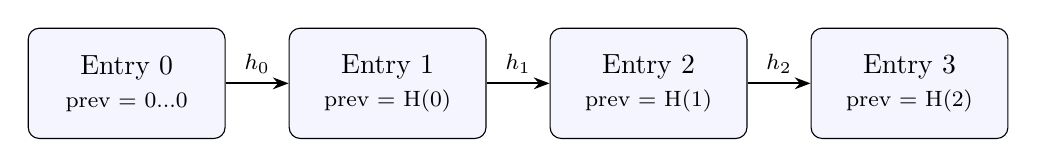
\begin{tikzpicture}[node distance=8mm,
  block/.style={draw,rounded corners,inner sep=4pt,align=center,fill=blue!4,minimum width=2.5cm,minimum height=1.4cm},
  arrow/.style={-{Stealth[length=2mm]}, thick}]
  \node[block] (e0) {Entry 0\\\footnotesize prev = 0...0};
  \node[block, right=of e0] (e1) {Entry 1\\\footnotesize prev = H(0)};
  \node[block, right=of e1] (e2) {Entry 2\\\footnotesize prev = H(1)};
  \node[block, right=of e2] (e3) {Entry 3\\\footnotesize prev = H(2)};
  \draw[arrow] (e0.east) -- node[above,font=\footnotesize]{$h_0$} (e1.west);
  \draw[arrow] (e1.east) -- node[above,font=\footnotesize]{$h_1$} (e2.west);
  \draw[arrow] (e2.east) -- node[above,font=\footnotesize]{$h_2$} (e3.west);
\end{tikzpicture}

\noindent
Why this is useful: if anyone tampers with entry 1 (changes a byte),
its hash $h_1$ changes. Entry 2's \texttt{prev\_hash} still claims the
old value, so the chain is broken. The auditor catches this in
$O(N)$ time during verification.

\begin{flagbox}[This is the ``blockchain-flavoured'' bit]
A hash chain is the data structure underneath Bitcoin's ``blockchain''.
We use the data structure --- not the rest of Bitcoin. There is no
proof-of-work, no mining, no currency, no consensus protocol. The
right reference is Certificate Transparency~\cite{RFC6962}, not
Bitcoin. See \cref{sec:notblockchain} for why we deliberately skip
PoW.
\end{flagbox}

\noindent
The entry hash $H(\text{entry})$ is computed over the
\emph{content fields only}, not over the signatures:

\[
  H(\text{entry}) = \mathsf{SHA256}\!\bigl(
    \mathtt{index} \,\|\, \mathtt{prev\_hash} \,\|\,
    \mathtt{timestamp} \,\|\, |\mathtt{payload}| \,\|\, \mathtt{payload}\bigr).
\]

\noindent
This means a cohort can collect more signatures on an entry over
time without changing the chain. Convenient for asynchronous signing
(\cref{sec:pending}).

\subsection{Record types}
\label{sec:records}

The \texttt{payload} of an entry is a JSON object with a \texttt{kind}
field that identifies the record type. There are six:

\begin{table}[h]
\centering\small
\begin{tabularx}{\textwidth}{l X}
\toprule
Kind & Content \\
\midrule
\textsf{ElectionSetup} & Genesis entry. Election ID (32 random bytes,
also used as the OTRS issue $I$), title, options, schedule, cohort
public keys, threshold $t$, optional witness keys and threshold $k$. \\
\textsf{VoterRegistration} & A voter's OTRS public key plus a
human-readable handle. \\
\textsf{RingPublication} & The ordered ring of all registered voter
pks. After this, registration is closed and voting opens. \\
\textsf{Ballot} & A voter's choice (one of the options) together with
their OTRS signature. \\
\textsf{VotingClosed} & A marker. No ballots may appear after this. \\
\textsf{TallyPublication} & The cohort's claimed final tally. Anyone
can recompute and refute. \\
\bottomrule
\end{tabularx}
\end{table}

\noindent
Code: \file{voting/records.py}. Each kind is a Python dataclass with
\texttt{to\_payload} / \texttt{from\_obj} methods. The polymorphic
parser \texttt{parse\_payload} dispatches by \texttt{kind}.

\subsection{The state machine}
\label{sec:fsm}

The legal sequence of records is

\[
  \textsf{Setup} \;\to\; (\textsf{Registration})^* \;\to\;
  \textsf{Ring} \;\to\; (\textsf{Ballot})^* \;\to\;
  \textsf{Closed} \;\to\; (\textsf{Tally})?
\]

\begin{center}
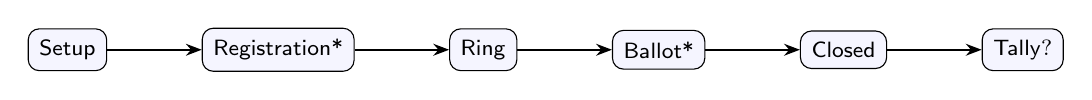
\begin{tikzpicture}[node distance=12mm,
  state/.style={draw,rounded corners,inner sep=4pt,fill=blue!4,font=\footnotesize},
  arrow/.style={-{Stealth[length=2mm]}, thick}]
  \node[state] (S) {\textsf{Setup}};
  \node[state, right=of S] (R) {\textsf{Registration*}};
  \node[state, right=of R] (G) {\textsf{Ring}};
  \node[state, right=of G] (B) {\textsf{Ballot*}};
  \node[state, right=of B] (C) {\textsf{Closed}};
  \node[state, right=of C] (T) {\textsf{Tally}?};
  \draw[arrow] (S) -- (R); \draw[arrow] (R) -- (G);
  \draw[arrow] (G) -- (B); \draw[arrow] (B) -- (C);
  \draw[arrow] (C) -- (T);
\end{tikzpicture}
\end{center}

\noindent
The auditor enforces this regex by walking the log linearly and
keeping a state variable. Any out-of-order record is rejected. The
state machine is the simplest possible enforcement of ``ballots after
ring, no ballots after close''.

% ===========================================================================
\section{Decentralisation}
\label{sec:dec}
% ===========================================================================

The system described so far has one weak spot: ``the organiser''.
What if the organiser:

\begin{itemize}[leftmargin=*]
  \item refuses to publish (the election stalls);
  \item goes offline (the election stalls);
  \item gets compromised (the attacker rewrites the result);
  \item lies about the tally (we catch them at audit, but it took us
    months to set up an election that's now invalid).
\end{itemize}

\noindent
Real elections solve this with \emph{multiple organisers} and rules
of the form ``any decision requires the agreement of at least $t$
of them''. We do the same digitally.

\subsection{The publisher cohort: $t$-of-$N$}
\label{sec:cohort}

Instead of one organiser with one Ed25519 key, we have a
\emph{cohort} of $N$ organisers, each holding their own key. Every
log entry must be co-signed by at least $t$ distinct cohort members
to be valid.

\begin{lstlisting}[style=pseudo]
ElectionSetup pins:
  cohort_pks = [$\pk_0$, $\pk_1$, ..., $\pk_{N-1}$]
  threshold  = $t$

Entry has:
  publisher_sigs = [($i_1$, $\sigma_1$), ($i_2$, $\sigma_2$), ...]
              # at least $t$ distinct indices, each sig valid under cohort_pks[$i$]
\end{lstlisting}

\noindent
This gives us two guarantees:

\begin{itemize}[leftmargin=*]
  \item \textbf{Liveness against $N - t$ unavailable members.}
    Up to $N - t$ cohort members can be offline or refusing to
    cooperate; the remaining $t$ can still proceed.
  \item \textbf{Soundness against $t - 1$ corrupted members.}
    A minority faction smaller than $t$ cannot append on its own.
\end{itemize}

\noindent
Common configurations:

\begin{table}[h]
\centering\small
\begin{tabular}{lll}
\toprule
$t$-of-$N$ & tolerates offline & tolerates corrupt \\
\midrule
2-of-3 & 1 & 1 \\
3-of-5 & 2 & 2 \\
4-of-7 & 3 & 3 \\
7-of-10 & 3 & 6 \\
\bottomrule
\end{tabular}
\end{table}

\noindent
Pick a configuration that matches your trust model: larger $t$ trades
liveness for soundness.

\paragraph{Asynchronous signing.}
Cohort members typically live on different machines. The
\emph{pending-entry} protocol lets them sign over time:

\begin{enumerate}[leftmargin=*]
  \item Any cohort member calls \texttt{propose\_entry(log, payload)}
    to create a sidecar file \file{<log>.pending}.
  \item Each cohort member, in any order, calls
    \texttt{cosign\_pending} to add their signature to the sidecar.
  \item Once the sidecar has $\ge t$ signatures, anyone calls
    \texttt{commit\_pending} to move it into the main log.
\end{enumerate}

\label{sec:pending}\noindent
Code: \file{voting/log.py}. CLI: \texttt{evote propose},
\texttt{evote sign-pending}, \texttt{evote commit-pending}.

\subsection{The witness federation: $k$-of-$M$}
\label{sec:witnesses}

The cohort layer protects against a corrupt minority. What if a
corrupt \emph{majority} ($\ge t$ malicious members) collude to publish
two different versions of the log to different observers?

This is called \emph{equivocation}. Cohort signatures alone cannot
prevent it (the colluding majority has enough signing power). The
classical fix is to add an \emph{independent} set of read-only
checkers: \emph{witnesses}.

A witness has their own Ed25519 keypair. Their job is to:

\begin{enumerate}[leftmargin=*]
  \item Fetch the bulletin board.
  \item Verify it from scratch under the cohort identity.
  \item Emit a signed \emph{checkpoint} attesting to what they saw:
    ``at index $i$, the head hash is $h$''.
\end{enumerate}

\begin{lstlisting}[style=pseudo]
Checkpoint = (log_index, head_hash, witness_index, sig)
sig = Ed25519.Sign(witness_sk, "otrs-witness-checkpoint-v1" || log_index || head_hash || witness_index)
\end{lstlisting}

\noindent
Checkpoints accumulate in a sidecar file \file{<log>.witnesses}.

\paragraph{What property does this buy us?} If a corrupted majority
shows two different logs to two different honest witnesses, the two
checkpoints they emit will have the \emph{same log\_index} but
\emph{different head\_hash}. Anyone who collects both checkpoints has
public, undeniable proof that the cohort split. The auditor surfaces
this as \texttt{EQUIVOCATION}, and the election is invalidated.

\paragraph{What the auditor requires.} If the setup declared
witnesses, the auditor:

\begin{itemize}[leftmargin=*]
  \item verifies every checkpoint's signature;
  \item checks that no two checkpoints sign the same index with
    different hashes (no equivocation);
  \item requires at least $k$ distinct witnesses to have co-signed
    \emph{some} log index (the \emph{witness threshold}).
\end{itemize}

\noindent
Code: \file{voting/witness.py}. CLI: \texttt{evote witness-keygen},
\texttt{evote witness-checkpoint}.

% ===========================================================================
\section{The principals}
\label{sec:principals}
% ===========================================================================

Four kinds of party in the system:

\begin{description}[leftmargin=*]
  \item[Cohort member.] Holds one Ed25519 secret key. Can propose,
    co-sign, and commit entries to the main log. Trusted (with the
    rest of the cohort) to not collude past the threshold.
    Code: \file{voting/manager.py}.
  \item[Voter.] Holds one Ristretto255 OTRS secret key. Can read the
    log, build a ballot, and submit it. Identity is verified
    out-of-band by the cohort during registration; after that the
    voter's actions are anonymous within the ring.
    Code: \file{voting/voter.py}.
  \item[Witness.] Holds one Ed25519 secret key. Cannot write to the
    main log. Periodically fetches, verifies, and emits checkpoints
    to the witness sidecar. Code: \file{voting/witness.py}.
  \item[Auditor.] Anyone. Read-only. Holds no keys. Bootstraps the
    cohort and witness identities from the Setup entry, then runs the
    audit pipeline. Code: \file{voting/auditor.py}.
\end{description}

\begin{center}
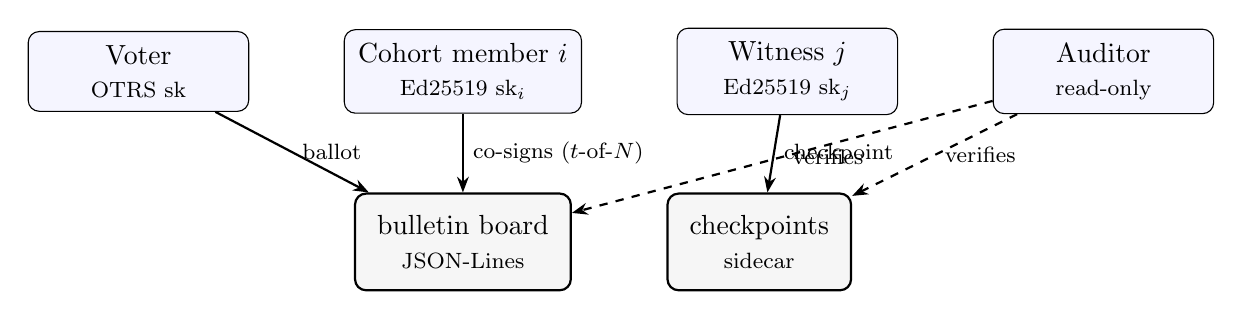
\begin{tikzpicture}[
  node distance=4mm and 12mm,
  block/.style={draw,rounded corners,inner sep=5pt,align=center,fill=blue!4,minimum width=2.8cm},
  arrow/.style={-{Stealth[length=2mm]}, thick},
  rwarrow/.style={-{Stealth[length=2mm]}, thick, dashed},
  store/.style={draw,thick,rounded corners,fill=gray!7,inner sep=8pt,align=center}
]
\node[block] (V) {Voter\\\footnotesize OTRS sk};
\node[block, right=of V] (Co) {Cohort member $i$\\\footnotesize Ed25519 sk$_i$};
\node[block, right=of Co] (W) {Witness $j$\\\footnotesize Ed25519 sk$_j$};
\node[block, right=of W] (A) {Auditor\\\footnotesize read-only};

\node[store, below=10mm of Co] (BB) {bulletin board\\\footnotesize JSON-Lines};
\node[store, right=of BB] (CP) {checkpoints\\\footnotesize sidecar};

\draw[arrow] (V) -- node[right,font=\footnotesize]{ballot} (BB);
\draw[arrow] (Co) -- node[right,font=\footnotesize]{co-signs ($t$-of-$N$)} (BB);
\draw[arrow] (W) -- node[right,font=\footnotesize]{checkpoint} (CP);
\draw[rwarrow] (A) -- node[right,font=\footnotesize]{verifies} (BB);
\draw[rwarrow] (A) -- node[right,font=\footnotesize]{verifies} (CP);
\end{tikzpicture}
\end{center}

\noindent
Voters do not need to know who the cohort members are by name; they
need only the cohort \emph{public keys}, which they read from the
genesis Setup entry. Auditors do not need any private state; they
only need the log files.

% ===========================================================================
\section{The audit algorithm}
\label{sec:audit}
% ===========================================================================

The single most important function in the project is
\texttt{voting.auditor.audit}. It is what makes ``verifiable''
actually true. It runs in seven steps. If any check fails it raises
\texttt{AuditError} and the election is invalid.

\paragraph{Step 1: bootstrap.}
Parse entry 0 as an \textsf{ElectionSetup}. Extract:
the election ID, the cohort pks, the threshold $t$, the witness pks,
the witness threshold $k$. All subsequent checks use this Setup as
ground truth.

\paragraph{Step 2: chain integrity.}
For every entry $i = 0, 1, 2, \ldots$:
\begin{itemize}[leftmargin=*]
  \item the index field equals $i$;
  \item \texttt{prev\_hash} equals the SHA-256 of entry $i - 1$
    (or all zeros for $i = 0$);
  \item there are $\ge t$ distinct signer indices in
    \texttt{publisher\_sigs}, and every signature verifies under the
    cohort key at the claimed index;
  \item the timestamp is $\ge$ the previous entry's timestamp.
\end{itemize}

\paragraph{Step 3: state-machine.}
Walk the entries enforcing the regex of \cref{sec:fsm}. Any record
out of state is rejected.

\paragraph{Step 4: per-record validity.}
\begin{itemize}[leftmargin=*]
  \item Every voter pk in a \textsf{VoterRegistration} record must be
    a valid Ristretto255 group element.
  \item The \textsf{RingPublication}'s ring must be exactly the
    multiset of voter pks in the prior \textsf{VoterRegistration}
    records (no extras, no missing).
  \item Every \textsf{Ballot}'s choice must appear in the
    \textsf{ElectionSetup} options.
  \item Every ballot's OTRS signature must verify against the
    election ID and the ring.
  \item Ballot timestamps must lie within
    $[\texttt{voting\_open}, \texttt{voting\_close}]$.
\end{itemize}

\paragraph{Step 5: witness federation (if declared).}
\begin{itemize}[leftmargin=*]
  \item Every checkpoint's signature verifies under the claimed
    witness key.
  \item No two checkpoints sign the same index with different
    head hashes (no \texttt{EQUIVOCATION}).
  \item At least $k$ distinct witnesses must agree on at least one
    index.
\end{itemize}

\paragraph{Step 6: tally.}
For each ballot $k$ compute the OTRS column vector
$(\sigma_1^{(k)}, \ldots, \sigma_n^{(k)})$ from its signature points
$A_0^{(k)}, A_1^{(k)}$. Then:

\begin{itemize}[leftmargin=*]
  \item Two ballots share a signer iff their column vectors collide
    at some position $j$.
  \item Group all ballots that share collision positions. Each group
    corresponds to one voter.
  \item If a group has one distinct choice, count it once.
  \item If a group has two or more distinct choices, that voter
    \emph{double-signed}: reject all of their ballots and emit their
    pk in the culprit list.
\end{itemize}

\noindent
The probability that two ballots by \emph{different} voters
spuriously share a column is bounded by $\binom{B}{2} \cdot 2^{-252}$
for $B$ ballots --- cryptographically negligible.

\paragraph{Step 7: tally claim verification.}
If the log contains a \textsf{TallyPublication}, compare the
auditor-computed tally to the cohort's claim. A mismatch fails the
audit. (The CLI exits non-zero, which a script can check.)

\paragraph{Output.}
An \texttt{AuditReport} object containing the canonical tally,
the per-ballot accepted/rejected status, the list of double-sign
culprit pks, and the witness-co-signing status. The CLI prints all
of this.

% ===========================================================================
\section{Worked example}
\label{sec:worked}
% ===========================================================================

A four-voter election run by three faculty cohort members and two
witnesses. Concrete file by file.

\paragraph{Setup.} Three Ed25519 keypairs for the cohort
(Profs.~Adami, Bianchi, Conti), threshold 2-of-3. Two for the
witnesses (Dean, Ombudsman), threshold 1-of-2 (loose for a small
demo). Four voters (Alice, Bob, Carol, Dave), each with their own
Ristretto255 OTRS keypair.

\paragraph{Entry 0 (genesis).}
\begin{lstlisting}[style=json]
{
  "index": 0, "prev_hash": "AAAA...", "timestamp": 1716580800,
  "payload": "<base64 of: {kind: election_setup, election_id: 'a4b2...',
              title: 'Cafeteria midnight closing', options: ['yes','no'],
              cohort_pks_b64: [Adami_pk, Bianchi_pk, Conti_pk], threshold: 2,
              witness_pks_b64: [Dean_pk, Ombuds_pk], witness_threshold: 1,
              registration_close: ..., voting_open: ..., voting_close: ...}>",
  "publisher_sigs": [
    {"i": 0, "sig": "<Adami's sig>"},
    {"i": 1, "sig": "<Bianchi's sig>"}
  ]
}
\end{lstlisting}

\paragraph{Entries 1--4 (registrations).}
Each is a \textsf{VoterRegistration} co-signed by two cohort members
(possibly a different pair per voter --- the subset can rotate).

\paragraph{Entry 5 (ring publication).}
The four voter pks, sorted by raw bytes, co-signed by two cohort
members.

\paragraph{Entries 6--9 (ballots).}
Each voter's OTRS-signed ballot. The cohort just adds it to the log
--- the cohort does not verify the OTRS signature here, because the
auditor will. (If they did, they'd reveal that they trusted the
voter; this way they don't even need to look at the ballot to publish
it.)

\paragraph{Entry 10 (voting closed).}
\textsf{VotingClosed} marker, co-signed by two cohort members.

\paragraph{Witness checkpoints.}
Dean and Ombudsman each independently fetch the log, verify the
chain, and emit a checkpoint at \texttt{(log\_index=10, head\_hash=H)}
signed under their own key. Both agree on the same $H$ --- the cohort
was honest about what the head looks like.

\paragraph{Audit output.}
\begin{lstlisting}[style=shell]
$ python3 -m voting.cli audit --log log.jsonl

election:               Cafeteria midnight closing
election_id:            a4b2...
cohort:                 2-of-3
witnesses:              1-of-2; valid checkpoints: 2; latest co-signed idx: 10
ring size:              4
accepted ballots:       4
rejected ballots:       0
tally:
  no              1
  yes             3
double-sign culprits:   0
\end{lstlisting}

\paragraph{What if Alice tried to vote twice?}
She signs two ballots with different choices. Both go on the log.
At audit time, OTRS Trace fires: Alice's column matches in both
ballots. Both ballots are rejected; Alice's pk is in the culprit list.
The link from pk to ``Alice the human'' lives in her
\textsf{VoterRegistration} entry (handle ``alice''), so the cohort can
follow up; but the cryptography itself is at the pk level.

\paragraph{What if the cohort lies about the tally?}
They publish a \textsf{TallyPublication} with the wrong numbers.
The auditor recomputes from the actual ballots, finds the mismatch,
exits non-zero. The lie is publicly visible.

\paragraph{What if a corrupted majority equivocates?}
They show ledger A to the Dean and ledger B (with one ballot
different) to the Ombudsman. Both are validly cohort-signed. The
Dean signs \texttt{Checkpoint(idx=10, hash=A)}, the Ombudsman signs
\texttt{Checkpoint(idx=10, hash=B)}. Anyone who collects both
checkpoints sees the same index with two different hashes: undeniable
proof. The auditor raises \texttt{AuditError(``EQUIVOCATION'')}.

% ===========================================================================
\section{Architecture~B: the proof-of-work chain}
\label{sec:chain}
% ===========================================================================

So far every section has described Architecture~A --- the federated
bulletin board in \file{voting/}. The repository ships a second
architecture in \file{chain/} that uses the \emph{same} cryptography
(OTRS, exactly), the \emph{same} record types (\file{voting/records.py},
unchanged), and the \emph{same} audit algorithm for the tally step
--- but replaces the cohort-signed log with a Bitcoin-shaped
proof-of-work chain. The point of building both is to make the
trade-off concrete, not theoretical: with the same primitive
underneath, what does the storage layer actually buy you?

This section walks through the chain at the same intuition-then-math
pace as the rest of the notes. If you understood A, B will feel like
a swap of one building block --- the storage layer --- with the rest
of the structure preserved.

\begin{intuition}
A chain is the same idea as the bulletin board (an append-only,
hash-chained record), with two differences that come from the
cryptocurrency lineage: (i) anyone can append, but appending is
\emph{costly} (you have to solve a puzzle); (ii) there is an
internal token economy --- eVotes --- so that the people doing the
appending (\emph{miners}) get paid.
\end{intuition}

% ---------------------------------------------------------------------------
\subsection{The block format}
% ---------------------------------------------------------------------------

A block is a fixed 121-byte header plus a variable-length list of
transactions. The header is what gets hashed for the PoW puzzle:

\begin{center}\small
\begin{tabular}{ll}
\toprule
Field & Bytes \\
\midrule
\texttt{prev\_hash} (SHA-256 of parent's header) & 32 \\
\texttt{height} (big-endian) & 8 \\
\texttt{difficulty} (1 byte, $0$--$255$) & 1 \\
\texttt{timestamp} (Unix seconds, big-endian) & 8 \\
\texttt{miner\_pk} (Ed25519 raw) & 32 \\
\texttt{tx\_root} (SHA-256 of canonical tx bytes) & 32 \\
\texttt{nonce} (big-endian) & 8 \\
\bottomrule
\end{tabular}
\end{center}

The transactions themselves live alongside the header (not inside it).
They are committed to via \texttt{tx\_root}, which is the SHA-256 hash
of the concatenation of each transaction's canonical bytes. So if
anyone tampers with a transaction body, \texttt{tx\_root} no longer
matches and the block fails validation.

\begin{flagbox}
This is a Merkle-flat root, not a Merkle tree. Merkle trees buy you
\emph{inclusion proofs} (proving a specific tx is in a block without
sending the whole block). Our blocks are small enough that we ship
the whole tx list at audit time, so the simpler flat hash is
sufficient. Adding a Merkle tree is one of the obvious follow-ups
if you want light clients.
\end{flagbox}

% ---------------------------------------------------------------------------
\subsection{The PoW puzzle}
% ---------------------------------------------------------------------------

The proof-of-work requirement is the simplest possible:
\[
  \mathrm{leading\_zero\_bits}\bigl(\mathrm{SHA{-}256}(\text{header})\bigr)
  \;\geq\; \text{difficulty}.
\]
The \texttt{nonce} field of the header is the only thing the miner
mutates; they try nonce $= 0, 1, 2, \ldots$ until the hash has enough
leading zeros.

\begin{intuition}
SHA-256 is unpredictable: changing the nonce by 1 produces a hash
that looks completely different. With probability $2^{-d}$ a random
nonce produces a hash with $d$ leading zero bits. So mining at
difficulty $d$ takes on average $2^d$ tries.
\end{intuition}

For the test suite we pin difficulty at 4--8 bits ($16$--$256$
expected hashes per block, sub-millisecond mining time on a laptop).
For a production deployment Bitcoin-style difficulty would be
$\approx 80$~bits ($10^{24}$ hashes per block, infeasible on a
single CPU). The \emph{difficulty adjustment} rule (in
\file{chain/mining.py}) bumps difficulty up or down by 1 if the
median inter-block interval over the last $11$ blocks falls outside
$[0.5T, 1.5T]$ around a target $T = 60$~seconds. This is exactly
the legacy node's logic from before this rewrite.

\paragraph{Cost vs.\ difficulty (measured).}
On the bench machine the single-process Python miner sustains
$\approx 270{,}000$ SHA-256 hashes per second:
\begin{center}\small
\begin{tabular}{rrr}
\toprule
$d$ & expected hashes & mine time / block \\
\midrule
4  & 16     & $0.09$~ms  \\
8  & 256    & $0.95$~ms  \\
12 & 4\,096  & $12.6$~ms  \\
16 & 65\,536 & $264.6$~ms \\
\bottomrule
\end{tabular}
\end{center}
A native (Rust/C) miner on the same hardware would hit $\sim 50$M
hashes per second --- $\sim 200{,}000\times$ faster --- but the cost
\emph{ratio} between honest miners and any attacker is the same, and
that ratio is what the security analysis turns on.

% ---------------------------------------------------------------------------
\subsection{The eVote ledger}
% ---------------------------------------------------------------------------

Every Ed25519 public key has an \emph{account}:
\[
  \mathit{Account} = (\mathit{balance},\ \mathit{nonce}).
\]
\texttt{balance} is the eVote balance, an unsigned integer.
\texttt{nonce} is the number of transactions this account has sent so
far. The next transaction sent by this account \emph{must} have
\texttt{nonce} equal to the account's current nonce; after applying
the tx the account's nonce increments by 1. This is the standard
account-model replay defence (Ethereum uses the same).

\begin{flagbox}
Why not UTXO (Bitcoin's model)? UTXO is better for parallelism and
fungibility analysis; account is far simpler in Python and matches
our use case (mostly account-to-miner fee flows, no anonymity
plumbing). For an OTRS-voting prototype the win from UTXO is
negligible.
\end{flagbox}

The genesis block contains zero or more \texttt{coinbase}
transactions that mint initial allocations. After that:
\begin{itemize}[leftmargin=*]
  \item Each non-genesis block contains \emph{exactly one}
        \texttt{coinbase} as its first transaction;
  \item The coinbase amount must equal
        $\mathit{block\_reward} + \sum \mathit{fees}$ across all
        other transactions in the block;
  \item Any other transaction failing validation rejects the entire
        block (state changes are atomic --- the block is applied on
        a snapshot, committed only on success).
\end{itemize}

% ---------------------------------------------------------------------------
\subsection{The eight transaction kinds}
% ---------------------------------------------------------------------------

Two are \emph{plumbing} (move eVotes around), six \emph{wrap the
voting record types} you already know from \cref{sec:records}.

\begin{center}\small
\begin{tabular}{lll}
\toprule
Kind & Signed by & Wraps \\
\midrule
\texttt{coinbase}        & --- (per-block, first tx) & mints reward + fees \\
\texttt{transfer}        & sender                    & --- (eVote payment) \\
\texttt{setup\_poll}     & poll creator              & \textsf{ElectionSetup} \\
\texttt{register\_voter} & sponsor                   & \textsf{VoterRegistration} \\
\texttt{publish\_ring}   & poll creator              & \textsf{RingPublication} \\
\texttt{ballot}          & \emph{none}               & \textsf{Ballot} \\
\texttt{close\_poll}     & poll creator              & \textsf{VotingClosed} \\
\texttt{tally}           & poll creator              & \textsf{TallyPublication} \\
\bottomrule
\end{tabular}
\end{center}

\begin{flagbox}[Issue]
\textbf{Ballots are the only unsigned kind.} They have no
chain-layer sender, no Ed25519 signature, and pay no fee. This is
\emph{essential} for anonymity: a fee-bearing or
sender-bearing ballot would expose the voter's identity on chain.
The validity check is purely the OTRS signature inside the ballot
payload, which anyone can verify against the published ring.

The cost of this design is that miners receive no per-ballot
incentive --- they include ballots because the protocol rules say
they must. In a hostile network you would compensate miners via the
\emph{poll setup fee} (escrowed by the poll creator), but the
current prototype keeps the rule simple.
\end{flagbox}

% ---------------------------------------------------------------------------
\subsection{Validation rules}
% ---------------------------------------------------------------------------

For each kind, \file{chain/state.py} enforces:

\begin{itemize}[leftmargin=*]
  \item \texttt{transfer}: sender's nonce matches account, signature
        verifies under sender's pk, balance covers sum-of-recipients
        plus fee.
  \item \texttt{setup\_poll}: creator's nonce + signature + fee
        OK; the embedded \textsf{ElectionSetup} parses and validates;
        \texttt{election\_id} not already in use; creator becomes the
        named manager of the poll.
  \item \texttt{register\_voter}: sponsor's nonce + sig + fee OK;
        \texttt{election\_id} exists and is in
        \textsf{registration} phase; block timestamp before
        \texttt{registration\_close}; voter pk is a valid Ristretto
        point and not already registered.
  \item \texttt{publish\_ring}: creator's nonce + sig + fee OK;
        poll exists; \emph{caller is the poll creator}; ring set
        equals the set of registered voter pks.
  \item \texttt{ballot}: poll exists and is in \textsf{voting} phase;
        block timestamp in
        $[\texttt{voting\_open},\,\texttt{voting\_close}]$;
        \texttt{choice} in option set;
        OTRS signature verifies against the published ring.
  \item \texttt{close\_poll}, \texttt{tally}: creator-only; phase
        guards; \texttt{close\_poll} requires
        \texttt{block\_timestamp $\ge$ voting\_close}.
\end{itemize}

The poll-creator check is the chain's analogue of A's cohort: each
poll has a single accountable identity that can publish phase
transitions for it. The chain itself, however, is permissionless ---
anyone can mine the blocks.

% ---------------------------------------------------------------------------
\subsection{The chain audit}
\label{sec:chain-audit}
% ---------------------------------------------------------------------------

The audit pipeline for B is almost identical to A's
(\cref{sec:audit}), with one step swapped:

\begin{enumerate}[leftmargin=*]
  \item \textbf{Chain integrity.} Re-load the chain from disk. For
        each block: verify PoW, verify \texttt{prev\_hash} chains
        back, verify timestamps strictly increase, verify
        \texttt{tx\_root} matches transactions, run
        \texttt{apply\_block} (which re-validates every signature,
        every nonce, every balance, every state-machine transition,
        and OTRS-verifies every ballot). \emph{This is the step that
        differs from A; the rest is identical.}
  \item \textbf{Per-poll tally.} For each poll in the resulting
        state, run the same $\sigma$-column algorithm as in
        \cref{sec:audit}: bucket every ballot's column tags, identify
        any signer who appears in two ballots with different choices
        (double-sign), aggregate the rest into the tally.
  \item \textbf{Compare against any on-chain
        \textsf{TallyPublication}}: if present and the numbers
        disagree, the poll creator is lying. Audit exits non-zero.
\end{enumerate}

By the time step (1) completes, the chain has been re-validated end
to end; if you trust the result of step (1), the only remaining
question is the tally, and that is deterministic from the ballots.

% ---------------------------------------------------------------------------
\subsection{A chain-side worked example}
\label{sec:chain-example}
% ---------------------------------------------------------------------------

Same cast of characters as \cref{sec:worked}: Alice, Bob, Carol, with
the addition of Mallory the miner. Three blocks per phase, one
transaction per block (the CLI's convention):

\begin{enumerate}[leftmargin=*]
  \item \textbf{Genesis.} Mallory's node starts a chain. The genesis
        block contains a coinbase that mints $1000$~eVotes to Alice
        (the project sponsor). Height $0$. No PoW needed for genesis
        --- there is no parent to anchor to.

  \item \textbf{Setup.} Alice broadcasts a \texttt{setup\_poll}
        transaction containing the \textsf{ElectionSetup} payload
        (title ``Best Lunch'', options ``pasta / pizza /
        \textit{focaccia}'', timestamps). Fee: 5 eVotes. Mallory
        mines a block at height $1$ containing this tx plus a
        coinbase for $50 + 5 = 55$~eVotes to herself. The PoW puzzle
        is satisfied; Mallory broadcasts the block.

  \item \textbf{Three registrations.} Alice broadcasts three
        \texttt{register\_voter} transactions (one per voter pk, fee
        $1$ each). Mallory mines three blocks at heights $2, 3, 4$.
        Alice's balance is now $1000 - 5 - 3 = 992$.

  \item \textbf{Ring publication.} Alice's
        \texttt{publish\_ring} tx freezes the ordered ring; mined
        into block~$5$. From this point the poll is in the
        \textsf{voting} phase; ballots become valid.

  \item \textbf{Three ballots.}
        \emph{Each voter} now broadcasts a \texttt{ballot}
        transaction --- unsigned at the chain layer, OTRS-signed
        inside the payload. Mallory mines blocks $6$, $7$, $8$
        containing one ballot each. The ballots travel over the
        public network; their \emph{contents} are public; but
        anonymity inside the ring of three still holds because the
        OTRS signature does not identify the signer, and there is
        no Ed25519 wrapper sender.

  \item \textbf{Close.} Alice broadcasts \texttt{close\_poll} once
        the voting window passes; mined into block~$9$.

  \item \textbf{Audit.} Anyone with the chain file can run
        \texttt{python3 -m chain.cli audit --chain c.bin}.
        The replay confirms PoW + state-machine + OTRS-per-ballot;
        the $\sigma$-column tally counts $2$ pasta vs.\ $1$ pizza;
        no \textsf{TallyPublication} present, so the audit just
        prints the result.
\end{enumerate}

\paragraph{Double-sign on chain.} If Bob tries to vote twice
(perhaps Mallory accepts the second tx into a later block), Bob's
two ballots both verify individually, but the auditor's
$\sigma$-column algorithm sees the same column tag appearing in two
ballots with different \texttt{choice} values. Both Bob ballots are
discarded; Bob's OTRS public key is surfaced in the audit report.
The trace algorithm is identical to A's --- it depends only on the
ballots, not on how they were ordered.

\paragraph{Equivocation on chain.} The chain has no analogue of A's
\emph{witness federation}. The cheapest defence is the
longest-chain rule itself: a $\geq 51\%$ miner can rewrite recent
blocks (a \emph{reorg}). Long-range reorgs of an abandoned chain
are not even cheap --- they are free. This is the structural
weakness B inherits from PoW.

% ---------------------------------------------------------------------------
\subsection{When each architecture wins}
\label{sec:notblockchain}
% ---------------------------------------------------------------------------

\paragraph{A wins when} the election has a known accountable
authority set --- a university senate, a corporate board, an
inter-institution treaty body. Finality is in seconds; there is no
token economy; operating cost is bounded to running $N + M$ named
parties. The cohort + witness model is the same one Certificate
Transparency, Sigsum~\cite{Sigsum2024}, and sigstore use for
similar problems.

\paragraph{B wins when} permissionless validator membership is a
non-negotiable design constraint --- no party, including the poll
creator, is trusted to host the canonical record. The chain has no
genesis-pinned trust set beyond the protocol rules; anyone with
hashpower can produce blocks.

\paragraph{Neither solves} coercion resistance (a voter who reveals
$x_i$ enables trace-tag matching in both systems), compromised
voter devices (a malicious client signs whatever it wants), or
post-quantum security. These live upstream of the storage layer.

\paragraph{Where B specifically loses.} Finality is probabilistic
(reorgs are always possible). There is no equivocation witness ---
if a $\geq 51\%$ miner rewrites history, no out-of-band cross-check
flags it. Most importantly: the security budget per unit time is
bounded by aggregate fees, while the attacker's payoff scales with
the largest poll on the chain at any moment. For elections of
serious political stakes, rented-hashpower attacks become
cost-effective even on a continuously-mined multi-poll chain. There
is a serious academic paper~\cite{ParkSpecter2021} on this; the
\texttt{chain/}-specific addendum in \texttt{paper/threat\_model.md}
\S7 quantifies the bound.

\paragraph{End-to-end cost (measured).} At $N=50$ voters,
Architecture~A finishes a full election ($N$ registrations,
ring publication, $N$ ballots, close, audit) in $\approx 1.1$~s and
produces a $324$~KB bulletin board. Architecture~B finishes the
same election in $\approx 3.0$~s and produces a $344$~KB chain. The
$\sim 1.6\times$ overhead and $\sim 6\%$ storage overhead come from
PoW plus full transaction validation per block. Full tables are in
the evaluation section of \texttt{paper/artifact.tex}.

% ===========================================================================
\section{Codebase map}
\label{sec:code}
% ===========================================================================

\begin{table}[h]
\centering\small
\begin{tabularx}{\textwidth}{l X}
\toprule
File & What's in it / when to read it \\
\midrule
\file{otrs/group.py}        & \texttt{Scalar}, \texttt{Point} dataclasses; arithmetic over Ristretto255. Read when touching the math. \\
\file{otrs/hash.py}         & RFC 9380 \texttt{expand\_message\_xmd}, \texttt{hash\_to\_group}, \texttt{hash\_to\_scalar}. \\
\file{otrs/otrs.py}         & \texttt{keygen}, \texttt{sign}, \texttt{verify}, \texttt{trace}. The math in \cref{sec:trace} maps line-for-line. \\
\file{otrs/serialize.py}    & Canonical byte encodings. Touch if you ever change a wire format. \\
\file{otrs/\_libsodium.py}  & cffi binding to libsodium ristretto255. The boundary to native code. \\
\file{voting/log.py}        & \texttt{Entry}, \texttt{BulletinBoard}, \texttt{PublisherCohort}, pending-entry helpers. \\
\file{voting/records.py}    & The six record types + canonical JSON. \\
\file{voting/manager.py}    & Cohort APIs: setup, register, ring, ballot, close, tally. \\
\file{voting/voter.py}      & Voter APIs: key import/export, ballot construction. \\
\file{voting/witness.py}    & \texttt{Checkpoint}, \texttt{emit\_checkpoint}, \texttt{verify\_checkpoints}. \\
\file{voting/auditor.py}    & \texttt{audit} --- the seven-step pipeline of \cref{sec:audit}. \\
\file{voting/cli.py}        & The \texttt{evote} command-line tool. \\
\file{tests/test\_otrs.py}  & 38 cryptographic tests (correctness + adversarial). \\
\file{tests/test\_log.py}   & 14 bulletin-board integrity tests. \\
\file{tests/test\_election.py} & 10 end-to-end election integration tests. \\
\file{tests/test\_threshold.py} & 12 tests for threshold cohort and witnesses (incl.\ equivocation). \\
\bottomrule
\end{tabularx}
\end{table}

\noindent
\textbf{Suggested first-pass reading order:} \file{otrs/otrs.py},
\file{voting/log.py}, \file{voting/records.py},
\file{voting/auditor.py}. Then the tests.

% ===========================================================================
\section{Dev environment}
% ===========================================================================

\begin{lstlisting}[style=shell]
sudo apt install -y libsodium23 python3-cffi python3-pytest \
    python3-hypothesis python3-cryptography texlive-latex-recommended

# from repo root
python3 -m pytest -v                                  # all 111 tests in <1s
python3 -m bench.bench_otrs --sizes 2,4,8,16,32,64    # OTRS microbench
make -C paper                                          # rebuild the artifact paper PDF
make -C docs                                           # rebuild THESE notes
\end{lstlisting}

\noindent
A copy-paste end-to-end CLI demo is in the project \texttt{README.md};
running it takes about 30 seconds.

% ===========================================================================
\section{Open problems --- where you would contribute}
\label{sec:open}
% ===========================================================================

In roughly increasing order of difficulty:

\begin{enumerate}[leftmargin=*]
  \item\label{itm:tamarin} \textbf{Tamarin / ProVerif model of the
    protocol layer.} Encode the state machine, the threshold cohort,
    and the witness federation as a process calculus and verify
    ballot anonymity + double-vote detection automatically. The
    state space is small. Estimated effort: 6--10 weeks. Output:
    a publishable artifact-track paper. \textbf{Highest
    value-to-effort ratio.}

  \item\label{itm:frost} \textbf{FROST threshold Ed25519.} Replace
    the per-entry vector of $t$ separate Ed25519 signatures with a
    single 64-byte FROST signature~\cite{FROST2020}. Drops storage
    by $64(t-1)$ bytes per entry. Engineering with real cryptography.
    Estimated effort: 8--12 weeks.

  \item\label{itm:gossip} \textbf{Gossip protocol for log +
    checkpoint replication.} The cohort and witnesses should each
    hold a copy of the log and the checkpoint sidecar, with a gossip
    protocol that anchors heads across peers. An escrowed secondary
    cohort that activates on timeout addresses the
    ``unanimously-malicious cohort'' liveness gap. Estimated
    effort: 12--16 weeks.

  \item\label{itm:browser} \textbf{Browser voter client.}
    The current CLI is fine for developers and ridiculous for real
    voters. A WebAssembly build of the OTRS signer plus a small webapp
    that submits to the cohort over HTTPS makes the voter side
    realistic. Estimated effort: 8--12 weeks.

  \item\label{itm:multi} \textbf{Multi-election bulletin board.}
    Currently one file equals one election. A registry of past
    elections, replicated across the cohort, makes long-running
    organisations (universities, unions) practical. Estimated effort:
    4--6 weeks.

  \item\label{itm:logsize} \textbf{Logarithmic-size traceable rings.}
    A signature is currently $O(n)$ bytes. A Groth--Kohlweiss
    one-out-of-many proof~\cite{GK15} would give $O(\log n)$ size
    for the membership step. Combining it with the trace tag $\sigma_i
    = h^{x_i}$ in a way that still allows \Trace{} to identify the
    position is, to our knowledge, \emph{open} in the literature.
    Estimated effort: 6--12 months and probably co-author work with
    a crypto researcher.

  \item\label{itm:receipt} \textbf{Receipt-freeness.} A voter who
    reveals $x_i$ to a coercer can prove their vote by recomputing
    $\sigma_i = h^{x_i}$ and matching it on-chain. The fix is a
    designated-verifier re-encryption layer \`a la
    JCJ~\cite{JCJ2005} or Civitas~\cite{Civitas2008}. Stacking it on
    OTRS is non-trivial because the trace tag is the very thing that
    breaks receipt-freeness. Estimated effort: 12--18 months.

  \item\label{itm:easycrypt} \textbf{EasyCrypt proofs of OTRS.}
    Re-prove the unforgeability / anonymity / traceability theorems
    of~\cite{ScafuroZhang2021} in EasyCrypt and link the proofs to
    the implementation via a code-extraction tool. Machine-checked
    security for the cryptographic core. Estimated effort: 6--9
    months with an EasyCrypt mentor.

  \item\label{itm:pq} \textbf{Post-quantum traceable ring.}
    The discrete-log security assumption falls to Shor's algorithm.
    Lattice-based linkable rings exist (Raptor~\cite{Raptor2018});
    extending to traceability with one-time tags is the hard part.
    Estimated effort: 12+ months, research project.
\end{enumerate}

\paragraph{Pick by goal.}
\begin{itemize}[leftmargin=*]
  \item Master's thesis aimed at a strong PhD program: item~\ref{itm:tamarin}
    or item~\ref{itm:easycrypt}.
  \item Industry security engineering: item~\ref{itm:frost}, \ref{itm:gossip}, or \ref{itm:browser}.
  \item Cryptography research career: item~\ref{itm:logsize} or item~\ref{itm:pq}, but get a co-advisor first.
\end{itemize}

% ===========================================================================
\section{Critical assessment: is it ``finally'' anonymous and verifiable?}
\label{sec:assessment}
% ===========================================================================

Short answer: \textbf{yes, in a precise technical sense}. Long answer:
you have to be able to recite the caveats. Both are in this section.

\subsection{The precise anonymity claim}

\textbf{What we provide.} Given the bulletin board, the published
ring $R = (\pk_1, \ldots, \pk_n)$, and one ballot's OTRS signature
$\sigma$ on message $m$ under issue $I$: no probabilistic
polynomial-time adversary can determine which $\pk_i \in R$ produced
$\sigma$ with probability non-negligibly better than $1/n$, assuming
the discrete-log problem is hard in Ristretto255 and the random-oracle
model holds for the hash functions.

\textbf{Where this breaks down.}

\begin{flaw}[Anonymity-set ceiling]
The anonymity set is the ring $R$. For $n = 4$ a single ballot is
hidden among four candidates --- if a coercer knows the other three
votes by other means, the fourth is exposed by elimination. Mitigation:
use larger rings.
\end{flaw}

\begin{flaw}[Registration is public]
The bulletin board lists every registered voter's pk and handle. So
``who registered'' is public. The anonymity is only over which option
each registered voter chose.
\end{flaw}

\begin{flaw}[No receipt-freeness]
A voter who reveals $x_i$ to a coercer can recompute
$\sigma_i = \Hzero(I \| R)^{x_i}$ and match it against the
$\sigma_j$ columns on each on-chain ballot to learn ``this is my
ballot''. This is the headline gap; see open problem~\ref{itm:receipt}.
\end{flaw}

\begin{flaw}[Network deanonymisation]
Submitting a ballot reveals source IP and timing. The system has no
built-in mitigation; voters would submit over Tor or a trusted relay
in a real deployment.
\end{flaw}

\begin{flaw}[Voter device compromise]
Malware with $\sk$ trivially impersonates the voter. Outside the
cryptographic scope --- needs hardware attestation.
\end{flaw}

\subsection{The precise verifiability claim}

\textbf{What we provide.} Given the bulletin board, the cohort public
keys, and (if declared) the witness public keys: any auditor can run
\texttt{evote audit} and:

\begin{enumerate}[leftmargin=*]
  \item Detect any tampering of the on-chain history.
  \item Verify every ballot was OTRS-valid against the published
    ring and election ID.
  \item Identify every voter who cast two distinct ballots and
    exclude their ballots from the tally.
  \item Recompute the official tally and refute any dishonest
    cohort claim.
  \item Detect any cohort equivocation, given honest witnesses.
\end{enumerate}

\noindent
The audit is \emph{deterministic} and \emph{public}: the same log
gives the same result for any auditor anywhere.

\textbf{Where this breaks down.}

\begin{flaw}[End-to-end voter inclusion]
A voter cannot cryptographically prove that \emph{their specific}
ballot was tallied without revealing their identity. They can
verify ``$N$ ballots tallied'', not ``mine was one of them''. The
literature solution is designated-verifier proofs, which conflict
with receipt-freeness.
\end{flaw}

\begin{flaw}[Cohort attestation is the eligibility oracle]
The cohort can attest any pk they want, including fake ones. The
cryptography cannot detect this --- it's an identity-proofing policy
problem. Mitigation: publicly observable registration, external
identity authority.
\end{flaw}

\begin{flaw}[Cohort controls timestamps]
A unanimous cohort can backdate ballots. Mitigations: witness
checkpoints inside the voting window, or an external time anchor
(Roughtime). Not in v0.3.
\end{flaw}

\begin{flaw}[Equivocation evidence needs multiple honest witnesses]
A single witness signing a divergent head is not enough. In a real
deployment $M$ should be moderately large (e.g., 5+) and witnesses
should be institutionally diverse.
\end{flaw}

\begin{flaw}[Censorship-evidence $\ne$ censorship-resistance]
v0.3 makes censorship publicly evident but cannot force the cohort
to publish. A unanimously malicious cohort stalls the election.
Fix: open problem~\ref{itm:gossip}.
\end{flaw}

\subsection{The honest pitch}

The sentence to defend in front of a security researcher:

\begin{quote}
\itshape
v0.3 is the cryptographic core of a verifiable anonymous voting
system, with the threshold-cohort and witness-federation layers that
the academic literature treats as necessary infrastructure;
receipt-freeness, censorship-resistance, and end-to-end voter-inclusion
remain open problems for v0.4 and beyond.
\end{quote}

If you can defend that sentence with the ten Issue boxes above, you
have understood the project.

% ===========================================================================
\appendix
\section{Glossary}
% ===========================================================================

\begin{description}[leftmargin=*,style=nextline]
  \item[anonymity set]
    The set of public keys among which a ring signature could plausibly
    have come from. Equals the ring.
  \item[audit]
    The deterministic verification of an election, performed by
    anyone with the bulletin board and the cohort/witness public
    keys. Implemented in \file{voting/auditor.py}.
  \item[ballot]
    A single voter's choice plus their OTRS signature, submitted as a
    record to the bulletin board.
  \item[bulletin board]
    The append-only JSON-Lines file where the election history lives.
    Each line is one entry.
  \item[checkpoint]
    A signed attestation by a witness of the form ``at log index $i$,
    the head hash is $h$''. Stored in a sidecar file.
  \item[cohort]
    The $N$ organisers of an election, each holding their own
    Ed25519 key. Any subset of size $\ge t$ can co-sign log entries.
  \item[discrete logarithm]
    The hard problem ``given $g$ and $g^x$, find $x$''. Our security
    rests on this being infeasible in Ristretto255.
  \item[Ed25519]
    The Ed25519 signature scheme. Used for cohort and witness
    signatures.
  \item[election ID]
    A 32-byte random hex string that uniquely identifies an election.
    Also serves as the OTRS \emph{issue} value.
  \item[entry]
    One line of the bulletin board: index, prev\_hash, timestamp,
    payload, publisher signatures.
  \item[equivocation]
    A cohort publishing two divergent versions of the log. Detected
    by the witness federation.
  \item[Fiat--Shamir]
    The trick of replacing an interactive protocol's random challenges
    by hashes of the transcript so far. Used inside OTRS.
  \item[group]
    A set with an associative, identity-having, inverse-having
    operation. Ristretto255 for us.
  \item[hash function]
    Deterministic recipe producing a fixed-size fingerprint. SHA-256
    for us.
  \item[hash chain]
    A sequence of entries each containing the hash of the previous.
    Makes the sequence tamper-evident.
  \item[hash-to-curve]
    Mapping arbitrary bytes deterministically into a group element.
    RFC~9380 instantiation for us.
  \item[issue]
    The OTRS election identifier. Equal to the election ID.
  \item[linked]
    Trace outcome when two ballots come from the same voter on the
    same message (a replay).
  \item[OTRS]
    One-time Traceable Ring Signature. The cryptographic primitive
    powering anonymous ballots with double-vote detection.
  \item[publisher cohort]
    Same as ``cohort''.
  \item[record]
    The typed JSON payload of a bulletin-board entry. Six kinds:
    Setup, Registration, Ring, Ballot, Closed, Tally.
  \item[ring]
    The ordered list of voter public keys for the OTRS scheme.
    Published after registration closes.
  \item[ring signature]
    A signature over a ring of public keys, proving ``one of these
    people signed'' without revealing which.
  \item[Ristretto255]
    A prime-order group of order $q \approx 2^{252}$ built on top of
    Curve25519. Our algebraic playground.
  \item[secret key / public key]
    The two halves of a public-key cryptographic identity. Secret
    stays private; public goes on the bulletin board.
  \item[threshold]
    The minimum number of cohort or witness members that must
    co-sign for validity ($t$ for cohort, $k$ for witnesses).
  \item[trace]
    The OTRS algorithm that compares two ballots and outputs
    ``independent'', ``linked'', or ``double-sign with culprit position''.
  \item[trace tag]
    The deterministic group element $\sigma_i = h^{x_i}$ embedded
    in every signature. Same voter on the same election always
    produces the same tag.
  \item[witness]
    An independent party who emits signed checkpoints attesting to
    the state of the bulletin board head.
\end{description}

\begin{thebibliography}{99}\small
\bibitem{ScafuroZhang2021} A.~Scafuro and B.~Zhang. One-time Traceable Ring Signatures. ESORICS, 2021.
\bibitem{RFC9380} S.~Scott, S.~Wood, R.~Wahby, A.~Faz-Hern\'andez, N.~Sullivan. Hashing to Elliptic Curves. RFC~9380, 2023.
\bibitem{FROST2020} C.~Komlo, I.~Goldberg. FROST: Flexible Round-Optimized Schnorr Threshold Signatures. SAC, 2020.
\bibitem{RFC6962} B.~Laurie, A.~Langley, E.~K\"asper. Certificate Transparency. RFC~6962, 2013.
\bibitem{Sigsum2024} R.~Berbain et al. Sigsum: Signed and verifiable software transparency. 2024.
\bibitem{GK15} J.~Groth and M.~Kohlweiss. One-Out-of-Many Proofs. EUROCRYPT, 2015.
\bibitem{JCJ2005} A.~Juels, D.~Catalano, M.~Jakobsson. Coercion-resistant electronic elections. WPES, 2005.
\bibitem{Civitas2008} M.~Clarkson, S.~Chong, A.~Myers. Civitas. IEEE S\&P, 2008.
\bibitem{Raptor2018} X.~Lu, M.~H.~Au, Z.~Zhang. Raptor: a Practical Lattice-Based (Linkable) Ring Signature. ACNS, 2019.
\bibitem{ParkSpecter2021} S.~Park, M.~Specter et al. Going from bad to worse: from Internet voting to blockchain voting. Journal of Cybersecurity, 2021.
\end{thebibliography}

\end{document}
